\section{Exercise eight}

A user request submitted to the system must wait in a memory queue before being processed in the central subsystem.
\begin{enumerate}
    \item With 100 active users, each with a 20-second think time, and a system response time of 10 seconds (the sum of memory queueing and central sub-system residence times), compute how many customers are, on average, competing for memory.
    \item If the memory queueing time is 8 seconds, compute the average number of customers loaded in memory.
\end{enumerate}

\subsection*{Solution}
The system is illustrated as follows:
\begin{figure}[H]
    \centering
    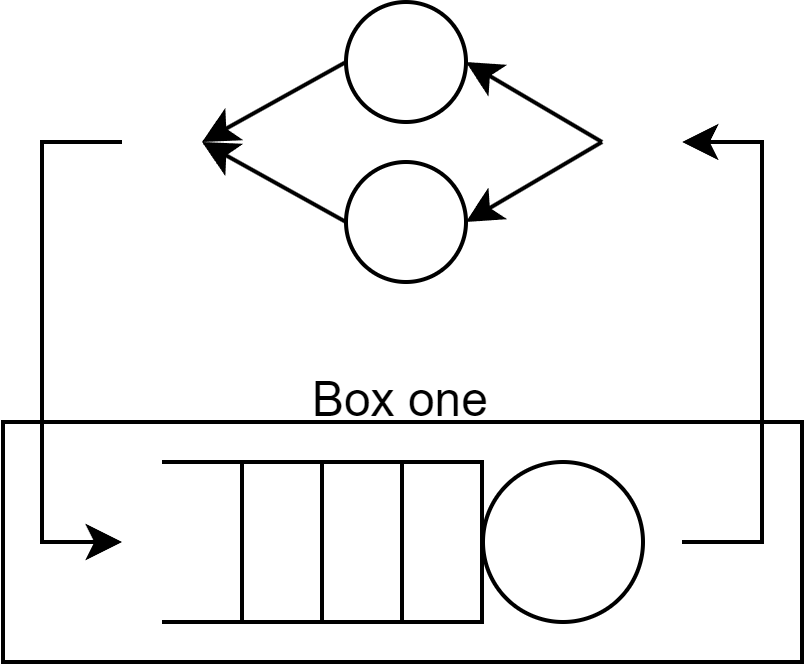
\includegraphics[width=0.35\linewidth]{images/per.png}
\end{figure}
Given:
\[N=100\qquad Z=20 \qquad R=10\]
\begin{enumerate}
    \item Using Little's law at the memory queue, we first calculate the system throughput:
        \[X=\dfrac{N}{R+Z}=\dfrac{100}{10+20}=3.3\]
        The number of users competing for memory:
        \[N_1=XR=3.3\cdot 10=33.3\]
    \item Given memory queueing response time $R_{mq}=8$, the number of users waiting in memory can be computed as:
        \[N_{cs}=N_1-N_{mq}=N_1-N_{mq}=33.3-3.3\cdot 8=6.6\]
\end{enumerate}